\begin{enumerate}[label=\thesection.\arabic*,ref=\thesection.\theenumi]
\item Write down a unit vector in XY-plane, making an angle of 30$^{\circ}$ with the positive direction of x-axis.\\
\item Find the scalar components and magnitude of the vector joining the points P($x_1,y_1,z_1 $) and Q ($x_2,y_2,z_2$ ).\\
\item A girl walks 4 km towards west, then she walks 3 km in a direction 30$^{\circ}$ east of north and stops. Determine the girl's displacement from her initial point of departure.\\
	\solution
		\iffalse
\documentclass[12pt]{article}
\usepackage{graphicx}
%\documentclass[journal,12pt,twocolumn]{IEEEtran}
\usepackage[none]{hyphenat}
\usepackage{graphicx}
\usepackage{listings}
\usepackage[english]{babel}
\usepackage{graphicx}
\usepackage{caption}
\usepackage[parfill]{parskip}
\usepackage{hyperref}
\usepackage{booktabs}
\usepackage{gensymb}
%\usepackage{setspace}\doublespacing\pagestyle{plain}
\def\inputGnumericTable{}
\usepackage{color}                                            %%
    \usepackage{array}                                            %%
    \usepackage{longtable}                                        %%
    \usepackage{calc}                                             %%
    \usepackage{multirow}                                         %%
    \usepackage{hhline}                                           %%
    \usepackage{ifthen}
\usepackage{array}
\usepackage{amsmath}   % for having text in math mode
\usepackage{parallel,enumitem}
\usepackage{listings}
\lstset{
language=tex,
frame=single,
breaklines=true
}
 
%Following 2 lines were added to remove the blank page at the beginning
\usepackage{atbegshi}% http://ctan.org/pkg/atbegshi
\AtBeginDocument{\AtBeginShipoutNext{\AtBeginShipoutDiscard}}
%
%New macro definitions
\newcommand{\mydet}[1]{\ensuremath{\begin{vmatrix}#1\end{vmatrix}}}
\providecommand{\brak}[1]{\ensuremath{\left(#1\right)}}
\providecommand{\norm}[1]{\left\lVert#1\right\rVert}
\newcommand{\solution}{\noindent \textbf{Solution: }}
\newcommand{\myvec}[1]{\ensuremath{\begin{pmatrix}#1\end{pmatrix}}}
\let\vec\mathbf
\begin{document}
\begin{center}
\enlargethispage{-4cm}
\title{\textbf{vector Algebra}}
\date{\vspace{-5ex}} %Not to print date automatically
\maketitle
\end{center}
\setcounter{page}{1}
\section*{12$^{th}$ Maths - Chapter 10}
This is Problem-3 from Exercise 10.4
\begin{enumerate}
\item A girl walks $4$ km towards west, then she walk $3$ km in a direction $30\degree$ east of north and stops. Determine the girl's displacement from her initial point of departure.

\solution 
\fi
		Let 
\begin{align}
	\vec{A}=\myvec{0\\0},
			\vec{B} -\vec{A}=\myvec{-4\\0},
	 \vec{C}-\vec{B}=\myvec{3\cos{60\degree}\\3\sin{60\degree}}
&=\myvec{\frac{3}{2}\\ \frac{3\sqrt{3}}{2}}
 \end{align}
 By triangle law of vector addition, 
\begin{align}
	\vec{C}-\vec{A} &= \vec{B}-\vec{A}+\vec{C}-\vec{B}\\
 &=\myvec{-4\\0}+\myvec{\frac{3}{2}\\[2pt] \frac{3\sqrt{3}}{2}}
=\myvec{\frac{-5}{2}\\[2pt] \frac{3\sqrt{3}}{2}}
\end{align}
which is the girl's displacement from her initial point of departure 
See Fig. 
\ref{fig:chapters/12/10/5/3Fig1}.
\begin{figure}[!h] 
 \begin{center} 
 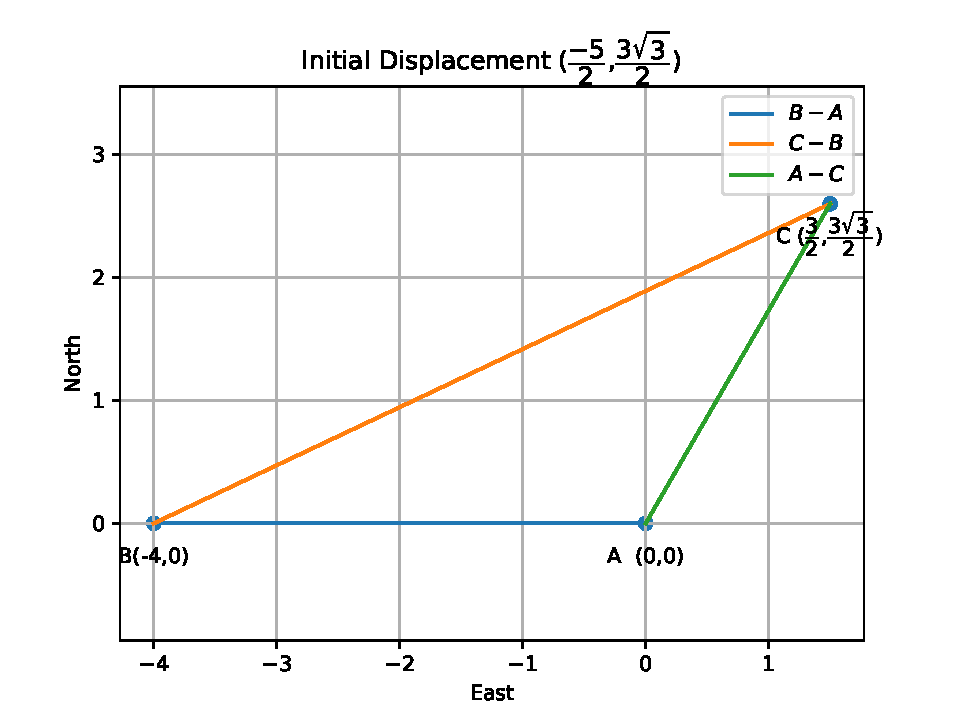
\includegraphics[width=\columnwidth]{chapters/12/10/5/3/figs/fig.pdf} 
 \end{center} 
\caption{} 
\label{fig:chapters/12/10/5/3Fig1} 
\end{figure}

\item If $\vec{a}=\vec{b}+\vec{c}$, then is it true that $|\vec{a}|=|\vec{b}|+|\vec{c}|$? Justify your answer.\\
	\solution
		\iffalse
\documentclass[journal,12pt,twocolumn]{IEEEtran}
\usepackage{graphicx}
\graphicspath{{./figs/}}{}
\usepackage{amsmath,amssymb,amsfonts,amsthm}
\newcommand{\myvec}[1]{\ensuremath{\begin{pmatrix}#1\end{pmatrix}}}
\providecommand{\norm}[1]{\lVert#1\rVert}
\usepackage{listings}
\usepackage{watermark}
\usepackage{titlesec}
\usepackage{caption}
\newcommand{\mydet}[1]{\ensuremath{\begin{vmatrix}#1\end{vmatrix}}}
\let\vec\mathbf
\lstset{
frame=single, 
breaklines=true,
columns=fullflexible
}
\thiswatermark{\centering \put(0,-105.0){
\includegraphics[scale=0.15]{/sdcard/IITH/vectors/12.10.5.4/figs/logo.png}} }
\title{\mytitle}
\title{
Assignment - 12.10.5.4
}
\author{Surajit Sarkar}
\begin{document}
\maketitle
\tableofcontents
\bigskip
\section{\textbf{Problem}}
if $\vec{a}=\vec{b}+\vec{c}$, then is true that $|\vec{a}|=|\vec{b}|+|\vec{c}|$?
Justify your answer .
\section{\textbf{Solution}}
Given
\begin{align}
    \vec{a}=\vec{b}+\vec{c}
\end{align}
\fi
Let
\begin{align}
    \vec{b}=\myvec{1\\2\\3},\vec{c}=\myvec{2\\-1\\-2}
\end{align}
Then
\begin{align}
	\vec{a}&=\vec{b}+\vec{c}
    =\myvec{3\\1\\1}
    \\
	\implies
    \norm{\vec{a}}
    &=\sqrt{11},\,
    \norm{\vec{b}}    =\sqrt{14},\,
    \norm{\vec{c}}
    =3.
\end{align}
Thus
\begin{align}
	\norm{\vec{a}}\ne\norm{\vec{b}}+\norm{\vec{c}}
\end{align}


\item Find the value of x for which $x(\hat{i}+\hat{j}+\hat{k})$ is a unit vector.\\
	\solution
		\iffalse
\documentclass[12pt]{article}
\usepackage{graphicx}
\usepackage[none]{hyphenat}
\usepackage{graphicx}
\usepackage{listings}
\usepackage[english]{babel}
\usepackage{graphicx}
\usepackage{caption} 
\usepackage{booktabs}
\usepackage{array}
\usepackage{amssymb} % for \because
\usepackage{amsmath}   % for having text in math mode
\usepackage{extarrows} % for Row operations arrows
\usepackage{listings}
\lstset{
  frame=single,
  breaklines=true
}
\usepackage{hyperref}
  
%Following 2 lines were added to remove the blank page at the beginning
\usepackage{atbegshi}% http://ctan.org/pkg/atbegshi
\AtBeginDocument{\AtBeginShipoutNext{\AtBeginShipoutDiscard}}


%New macro definitions
\newcommand{\mydet}[1]{\ensuremath{\begin{vmatrix}#1\end{vmatrix}}}
\providecommand{\brak}[1]{\ensuremath{\left(#1\right)}}
\providecommand{\norm}[1]{\left\lVert#1\right\rVert}
\newcommand{\solution}{\noindent \textbf{Solution: }}
\newcommand{\myvec}[1]{\ensuremath{\begin{pmatrix}#1\end{pmatrix}}}
\providecommand{\abs}[1]{\left\vert#1\right\vert}
\let\vec\mathbf

\begin{document}

\begin{center}
\title{\textbf{Equation  of Unit Vector}}
\date{\vspace{-5ex}} %Not to print date automatically
\maketitle
\end{center}
\setcounter{page}{1}
\section{12$^{th}$ Maths - Chapter 10}
\textbf{This is Problem-5 from Exercise 5.5}
\begin{enumerate}
\item Find the value of $x$ for which $x(\hat{i}+\hat{j}+\hat{k})$ is a unit vector
\section{Solution}
\solution
\fi
Let
\begin{align} 
\vec{x}&=x\myvec{1\\1\\1}
\implies
\norm{\vec{x}}=1
\\
\implies 
x\sqrt{3}&=1,\,
	\text{or, }x=\frac{1}{\sqrt{3}}
\end{align}   

\item Find a vector of magnitude 5 units, and parallel to the resultant of the vectors $\vec{a}=2\hat{i}+3\hat{j}-\hat{k}$ and $\vec{b}=\hat{i}-2\hat{j}+\hat{k}$.\\
\item If $\vec{a}=\hat{i}+\hat{j}+\hat{k}$,$\vec{b}=2\hat{i}-\hat{j}+3\hat{k}$ and $\vec{c}=\hat{i}-2\hat{j}+\hat{k}$, find a unit vector parallel to the vector $2\vec{a}-\vec{b}+3\vec{c}$.\\
	\solution
		\iffalse
\documentclass[10pt]{article}
\usepackage{graphicx}
\usepackage[none]{hyphenat}
\usepackage{graphicx}
\usepackage{listings}
\usepackage[english]{babel}
\usepackage{siunitx}
\usepackage{graphicx}
\usepackage{caption} 
\usepackage{booktabs}
\usepackage{array}
\usepackage{amssymb} % for \because
\usepackage{amsmath}   % for having text in math mode
\usepackage{extarrows} % for Row operations arrows
\usepackage{listings}
\usepackage[utf8]{inputenc}
\lstset{
  frame=single,
  breaklines=true
}
\usepackage{hyperref}
  
%Following 2 lines were added to remove the blank page at the beginning
\usepackage{atbegshi}% http://ctan.org/pkg/atbegshi
\AtBeginDocument{\AtBeginShipoutNext{\AtBeginShipoutDiscard}}


%New macro definitions
\newcommand{\mydet}[1]{\ensuremath{\begin{vmatrix}#1\end{vmatrix}}}
\providecommand{\brak}[1]{\ensuremath{\left(#1\right)}}
\newcommand{\solution}{\noindent \textbf{Solution: }}
\newcommand{\myvec}[1]{\ensuremath{\begin{pmatrix}#1\end{pmatrix}}}
\providecommand{\norm}[1]{\left\lVert#1\right\rVert}
\providecommand{\abs}[1]{\left\vert#1\right\vert}
\let\vec\mathbf{}
\begin{document}

\begin{center}
\title{\textbf{Vector Algebra}}
\date{\vspace{-5ex}} %Not to print date automatically
\maketitle
\end{center}

\section{12$^{th}$ Maths - Chapter 10}
This is Problem 7 from Exercise-10.5
\begin{enumerate}

\item If $\overrightarrow{a}=\hat{i}+\hat{j}+\hat{k}$,$\overrightarrow{b}=2\hat{i}-\hat{j}+3\hat{k}$ and $\overrightarrow{c}=\hat{i}-2\hat{j}+\hat{k}$, find a unit vector parallel to the vector $2\overrightarrow{a}-\overrightarrow{b}+3\overrightarrow{c}$.\\  

\solution
Given Vectors
\fi

\begin{align}
	\vec{u}=2\vec{a}-\vec{b}+3\vec{c}=\myvec{3\\-3\\2}
\implies
\hat{\vec{u}}=\frac{\vec{u}}{\norm{\vec{u}}}
=\frac{1}{\sqrt{22}}\myvec{3\\-3\\2}
\end{align}


\item Show that the points A (1, -2, -8), B (5, 0, -2) and C (11, 3, 7) are collinear, and find the ratio in which B divides AC.\\
\item Find the position vector of a point R which divides the line joining two points P and Q whose position vectors are $(2\vec{a}+\vec{b})$ and $(\vec{a}-3\vec{b})$
externally in the ratio 1 : 2. Also, show that P is the mid point of the line segment RQ.\\
\item The two adjacent sides of a parallelogram are 
$2\hat{i}-4\hat{j}+5\hat{k}$  and  $\hat{i}-2\hat{j}-3\hat{k}$.
Find the unit vector parallel to its diagonal. Also, find its area.\\
	\solution
		\iffalse
\documentclass[journal,12pt,twocolumn]{IEEEtran}
\usepackage{setspace}
\usepackage{gensymb}
\usepackage{xcolor}
\usepackage{caption}
\singlespacing
\usepackage{siunitx}
\usepackage[cmex10]{amsmath}
\usepackage{mathtools}
\usepackage{hyperref}
\usepackage{amsthm}
\usepackage{mathrsfs}
\usepackage{txfonts}
\usepackage{stfloats}
\usepackage{cite}
\usepackage{cases}
\usepackage{subfig}
\usepackage{longtable}
\usepackage{multirow}
\usepackage{enumitem}
\usepackage{bm}
\usepackage{mathtools}
\usepackage{listings}
\usepackage{tikz}
\usetikzlibrary{shapes,arrows,positioning}
\usepackage{circuitikz}
\renewcommand{\vec}[1]{\boldsymbol{\mathbf{#1}}}
\DeclareMathOperator*{\Res}{Res}
\renewcommand\thesection{\arabic{section}}
\renewcommand\thesubsection{\thesection.\arabic{subsection}}
\renewcommand\thesubsubsection{\thesubsection.\arabic{subsubsection}}

\renewcommand\thesectiondis{\arabic{section}}
\renewcommand\thesubsectiondis{\thesectiondis.\arabic{subsection}}
\renewcommand\thesubsubsectiondis{\thesubsectiondis.\arabic{subsubsection}}
\hyphenation{op-tical net-works semi-conduc-tor}

\lstset{
language=Python,
frame=single, 
breaklines=true,
columns=fullflexible
}
\begin{document}
\theoremstyle{definition}
\newtheorem{theorem}{Theorem}[section]
\newtheorem{problem}{Problem}
\newtheorem{proposition}{Proposition}[section]
\newtheorem{lemma}{Lemma}[section]
\newtheorem{corollary}[theorem]{Corollary}
\newtheorem{example}{Example}[section]
\newtheorem{definition}{Definition}[section]
\newcommand{\BEQA}{\begin{eqnarray}}
        \newcommand{\EEQA}{\end{eqnarray}}
\newcommand{\define}{\stackrel{\triangle}{=}}
\newcommand{\myvec}[1]{\ensuremath{\begin{pmatrix}#1\end{pmatrix}}}
\newcommand{\mydet}[1]{\ensuremath{\begin{vmatrix}#1\end{vmatrix}}}
\bibliographystyle{IEEEtran}
\providecommand{\nCr}[2]{\,^{#1}C_{#2}} % nCr
\providecommand{\nPr}[2]{\,^{#1}P_{#2}} % nPr
\providecommand{\mbf}{\mathbf}
\providecommand{\pr}[1]{\ensuremath{\Pr\left(#1\right)}}
\providecommand{\qfunc}[1]{\ensuremath{Q\left(#1\right)}}
\providecommand{\sbrak}[1]{\ensuremath{{}\left[#1\right]}}
\providecommand{\lsbrak}[1]{\ensuremath{{}\left[#1\right.}}
\providecommand{\rsbrak}[1]{\ensuremath{{}\left.#1\right]}}
\providecommand{\brak}[1]{\ensuremath{\left(#1\right)}}
\providecommand{\lbrak}[1]{\ensuremath{\left(#1\right.}}
\providecommand{\rbrak}[1]{\ensuremath{\left.#1\right)}}
\providecommand{\cbrak}[1]{\ensuremath{\left\{#1\right\}}}
\providecommand{\lcbrak}[1]{\ensuremath{\left\{#1\right.}}
\providecommand{\rcbrak}[1]{\ensuremath{\left.#1\right\}}}
\theoremstyle{remark}
\newtheorem{rem}{Remark}
\newcommand{\sgn}{\mathop{\mathrm{sgn}}}
\newcommand{\rect}{\mathop{\mathrm{rect}}}
\newcommand{\sinc}{\mathop{\mathrm{sinc}}}
\providecommand{\abs}[1]{\left\vert#1\right\vert}
\providecommand{\res}[1]{\Res\displaylimits_{#1}}
\providecommand{\norm}[1]{\lVert#1\rVert}
\providecommand{\mtx}[1]{\mathbf{#1}}
\providecommand{\mean}[1]{E\left[ #1 \right]}
\providecommand{\fourier}{\overset{\mathcal{F}}{ \rightleftharpoons}}
\providecommand{\ztrans}{\overset{\mathcal{Z}}{ \rightleftharpoons}}
\providecommand{\system}[1]{\overset{\mathcal{#1}}{ \longleftrightarrow}}
\newcommand{\solution}{\noindent \textbf{Solution: }}
\providecommand{\dec}[2]{\ensuremath{\overset{#1}{\underset{#2}{\gtrless}}}}
\let\StandardTheFigure\thefigure
\def\putbox#1#2#3{\makebox[0in][l]{\makebox[#1][l]{}\raisebox{\baselineskip}[0in][0in]{\raisebox{#2}[0in][0in]{#3}}}}
\def\rightbox#1{\makebox[0in][r]{#1}}
\def\centbox#1{\makebox[0in]{#1}}
\def\topbox#1{\raisebox{-\baselineskip}[0in][0in]{#1}}
\def\midbox#1{\raisebox{-0.5\baselineskip}[0in][0in]{#1}}

\vspace{3cm}
\title{12.10.5.10}
\author{Lokesh Surana}
\maketitle
\section*{Class 12, Chapter 10, Exercise 5.10}

Q.10. The two adjacent sides of a parallelogram are  ${2}\hat{i} -  {4}\hat{j} + {5}\hat{k}$ and ${1}\hat{i} -  {2}\hat{j} - {3}\hat{k}$.
Find the unit vector parallel to its diagonal. Also, find its area.

\solution 
\fi
Let the sides of the parallelogram be 
\begin{align}
\vec{a} = \myvec{2\\-4\\5}, \, \vec{b} = \myvec{1\\-2\\-3}.
\end{align}
The diagonals of the parallelogram are given by
\begin{align}
	\vec{D}_1 &= \vec{a} + \vec{b} = \myvec{3 \\-6\\2} \\
	\vec{D}_2 &= \vec{a} - \vec{b} = \myvec{1 \\-2\\8}
\end{align}
The unit vectors parallel to the diagonals are then given by
\begin{align}
	\hat{\vec{D}_1} &= \frac{\vec{D}_1}{\norm{\vec{D}_1}}  = \myvec{\frac{3}{\sqrt{45}}\\-\frac{6}{\sqrt{45}}\\\frac{2}{\sqrt{45}}} \\
    \hat{\vec{D}_2} &= \frac{\vec{D}_2}{\norm{\vec{D}_2}}  = \myvec{\frac{1}{\sqrt{69}}\\-\frac{2}{\sqrt{69}}\\\frac{8}{\sqrt{69}}}
\end{align}
%
Since
\begin{align}
    \vec{a}\times\vec{b}=\myvec{22 \\-11\\0},
\end{align}
he area of the parallelogram is given by
\begin{align}
    \norm{\vec{a}\times\vec{b}}  = \sqrt{605}
\end{align}


\item Show that the direction cosines of a vector equally inclined to the axes OX, OY and OZ are \textpm $\sbrak{\frac{1}{\sqrt{3}},\frac{1}{\sqrt{3}},\frac{1}{\sqrt{3}}}$.\\
	\solution
		\iffalse
\documentclass[journal,12pt,twocolumn]{IEEEtran}
%
\usepackage{setspace}
\usepackage{gensymb}
%\doublespacing
\singlespacing

%\usepackage{graphicx}
%\usepackage{amssymb}
%\usepackage{relsize}
\usepackage[cmex10]{amsmath}
%\usepackage{amsthm}
%\interdisplaylinepenalty=2500
%\savesymbol{iint}
%\usepackage{txfonts}
%\restoresymbol{TXF}{iint}
%\usepackage{wasysym}
\usepackage{amsthm}
%\usepackage{iithtlc}
\usepackage{mathrsfs}
\usepackage{txfonts}
\usepackage{stfloats}
\usepackage{bm}
\usepackage{cite}
\usepackage{cases}
\usepackage{subfig}
%\usepackage{xtab}
\usepackage{longtable}
\usepackage{multirow}
%\usepackage{algorithm}
%\usepackage{algpseudocode}
\usepackage{enumitem}
\usepackage{mathtools}
\usepackage{steinmetz}
\usepackage{tikz}
\usepackage{circuitikz}
\usepackage{verbatim}
\usepackage{tfrupee}
\usepackage[breaklinks=true]{hyperref}
%\usepackage{stmaryrd}
\usepackage{tkz-euclide} % loads  TikZ and tkz-base
%\usetkzobj{all}
\usetikzlibrary{calc,math}
\usepackage{listings}
    \usepackage{color}                                            %%
    \usepackage{array}                                            %%
    \usepackage{longtable}                                        %%
    \usepackage{calc}                                             %%
    \usepackage{multirow}                                         %%
    \usepackage{hhline}                                           %%
    \usepackage{ifthen}                                           %%
  %optionally (for landscape tables embedded in another document): %%
    \usepackage{lscape}     
\usepackage{multicol}
\usepackage{chngcntr}
%\usepackage{enumerate}

%\usepackage{wasysym}
%\newcounter{MYtempeqncnt}
\DeclareMathOperator*{\Res}{Res}
%\renewcommand{\baselinestretch}{2}
\renewcommand\thesection{\arabic{section}}
\renewcommand\thesubsection{\thesection.\arabic{subsection}}
\renewcommand\thesubsubsection{\thesubsection.\arabic{subsubsection}}

\renewcommand\thesectiondis{\arabic{section}}
\renewcommand\thesubsectiondis{\thesectiondis.\arabic{subsection}}
\renewcommand\thesubsubsectiondis{\thesubsectiondis.\arabic{subsubsection}}

% correct bad hyphenation here
\hyphenation{op-tical net-works semi-conduc-tor}
\def\inputGnumericTable{}                                 %%

\lstset{
%language=C,
frame=single, 
breaklines=true,
columns=fullflexible
}
%\lstset{
%language=tex,
%frame=single, 
%breaklines=true
%}

\begin{document}
%


\newtheorem{theorem}{Theorem}[section]
\newtheorem{problem}{Problem}
\newtheorem{proposition}{Proposition}[section]
\newtheorem{lemma}{Lemma}[section]
\newtheorem{corollary}[theorem]{Corollary}
\newtheorem{example}{Example}[section]
\newtheorem{definition}[problem]{Definition}
%\newtheorem{thm}{Theorem}[section] 
%\newtheorem{defn}[thm]{Definition}
%\newtheorem{algorithm}{Algorithm}[section]
%\newtheorem{cor}{Corollary}
\newcommand{\BEQA}{\begin{eqnarray}}
\newcommand{\EEQA}{\end{eqnarray}}
\newcommand{\define}{\stackrel{\triangle}{=}}

\bibliographystyle{IEEEtran}
%\bibliographystyle{ieeetr}


\providecommand{\mbf}{\mathbf}
\providecommand{\pr}[1]{\ensuremath{\Pr\left(#1\right)}}
\providecommand{\qfunc}[1]{\ensuremath{Q\left(#1\right)}}
\providecommand{\sbrak}[1]{\ensuremath{{}\left[#1\right]}}
\providecommand{\lsbrak}[1]{\ensuremath{{}\left[#1\right.}}
\providecommand{\rsbrak}[1]{\ensuremath{{}\left.#1\right]}}
\providecommand{\brak}[1]{\ensuremath{\left(#1\right)}}
\providecommand{\lbrak}[1]{\ensuremath{\left(#1\right.}}
\providecommand{\rbrak}[1]{\ensuremath{\left.#1\right)}}
\providecommand{\cbrak}[1]{\ensuremath{\left\{#1\right\}}}
\providecommand{\lcbrak}[1]{\ensuremath{\left\{#1\right.}}
\providecommand{\rcbrak}[1]{\ensuremath{\left.#1\right\}}}
\theoremstyle{remark}
\newtheorem{rem}{Remark}
\newcommand{\sgn}{\mathop{\mathrm{sgn}}}
\providecommand{\abs}[1]{\left\vert#1\right\vert}
\providecommand{\res}[1]{\Res\displaylimits_{#1}} 
\providecommand{\norm}[1]{\left\lVert#1\right\rVert}
%\providecommand{\norm}[1]{\lVert#1\rVert}
\providecommand{\mtx}[1]{\mathbf{#1}}
\providecommand{\mean}[1]{E\left[ #1 \right]}
\providecommand{\fourier}{\overset{\mathcal{F}}{ \rightleftharpoons}}
%\providecommand{\hilbert}{\overset{\mathcal{H}}{ \rightleftharpoons}}
\providecommand{\system}{\overset{\mathcal{H}}{ \longleftrightarrow}}
	%\newcommand{\solution}[2]{\textbf{Solution:}{#1}}
\newcommand{\solution}{\noindent \textbf{Solution: }}
\newcommand{\cosec}{\,\text{cosec}\,}
\providecommand{\dec}[2]{\ensuremath{\overset{#1}{\underset{#2}{\gtrless}}}}
\newcommand{\myvec}[1]{\ensuremath{\begin{pmatrix}#1\end{pmatrix}}}
\newcommand{\mydet}[1]{\ensuremath{\begin{vmatrix}#1\end{vmatrix}}}
%\numberwithin{equation}{section}
\numberwithin{equation}{subsection}
%\numberwithin{problem}{section}
%\numberwithin{definition}{section}
\makeatletter
\@addtoreset{figure}{problem}
\makeatother

\let\StandardTheFigure\thefigure
\let\vec\mathbf
%\renewcommand{\thefigure}{\theproblem.\arabic{figure}}
\renewcommand{\thefigure}{\theproblem}
%\setlist[enumerate,1]{before=\renewcommand\theequation{\theenumi.\arabic{equation}}
%\counterwithin{equation}{enumi}


%\renewcommand{\theequation}{\arabic{subsection}.\arabic{equation}}

\def\putbox#1#2#3{\makebox[0in][l]{\makebox[#1][l]{}\raisebox{\baselineskip}[0in][0in]{\raisebox{#2}[0in][0in]{#3}}}}
     \def\rightbox#1{\makebox[0in][r]{#1}}
     \def\centbox#1{\makebox[0in]{#1}}
     \def\topbox#1{\raisebox{-\baselineskip}[0in][0in]{#1}}
     \def\midbox#1{\raisebox{-0.5\baselineskip}[0in][0in]{#1}}

\vspace{3cm}


\title{Question: 12.10.5.11}
\author{Nikam Pratik Balasaheb (EE21BTECH11037)}





% make the title area
\maketitle

\newpage

%\tableofcontents

\bigskip

\renewcommand{\thefigure}{\theenumi}
\renewcommand{\thetable}{\theenumi}
%\renewcommand{\theequation}{\theenumi}

\section{Problem}
Show that direction cosines of a vector equally inclined to axes $ \vec{OX}, \vec{OY}$ and $\vec{OZ}$ are $\pm \myvec{\frac{1}{\sqrt{3}} \\[1pt] \frac{1}{\sqrt{3}} \\[1pt] \frac{1}{\sqrt{3}}} $
\section{Solution}
The vector is equally inclined to the axes $\vec{OX}$, $\vec{OY}$ and $\vec{OZ}$. Let the angle be $\theta$.
\fi

The direction vector can be expressed in terms of the direction cosines as 
\begin{align}
\vec{m}  = \myvec{\cos{\theta} \\ \cos{\theta} \\ \cos{\theta} }
\end{align}
Since 
\begin{align}
\norm{\vec{m}} = 1,
\abs{\sqrt{3} \cos{\theta}} =1 \implies
\cos{\theta} = \pm \frac{1}{\sqrt{3}}
\end{align}


\item Let $\vec{a}=\hat{i}+4\hat{j}+2\hat{k}$,$\vec{b}=3\hat{i}-2\hat{j}+7\hat{k}$ and $\vec{c}=2\hat{i}-\hat{j}+4\hat{k}$.Find a vector $\vec{d}$ which is perpendicular to both $\vec{a}$ and $\vec{b}$,and $\vec{c}.\vec{d}$=15.\\
	\solution
		\iffalse
\documentclass[journal,12pt,twocolumn]{IEEEtran}
\usepackage{setspace}
\usepackage{gensymb}
\singlespacing
\usepackage[cmex10]{amsmath}
\usepackage{amsthm}
\usepackage{mathrsfs}
\usepackage{txfonts}
\usepackage{stfloats}
\usepackage{bm}
\usepackage{cite}
\usepackage{cases}
\usepackage{subfig}
\usepackage{longtable}
\usepackage{multirow}
\usepackage{enumitem}
\usepackage{mathtools}
\usepackage{steinmetz}
\usepackage{tikz}
\usepackage{circuitikz}
\usepackage{verbatim}
\usepackage{tfrupee}
\usepackage[breaklinks=true]{hyperref}
\usepackage{tkz-euclide}
\usetikzlibrary{calc,math}
\usepackage{listings}
    \usepackage{color}                                            %%
    \usepackage{array}                                            %%
    \usepackage{longtable}                                        %%
    \usepackage{calc}                                             %%
    \usepackage{multirow}                                         %%
    \usepackage{hhline}                                           %%
    \usepackage{ifthen}                                           %%
  %optionally (for landscape tables embedded in another document): %%
    \usepackage{lscape}     
\usepackage{multicol}
\usepackage{chngcntr}
\DeclareMathOperator*{\Res}{Res}
\renewcommand\thesection{\arabic{section}}
\renewcommand\thesubsection{\thesection.\arabic{subsection}}
\renewcommand\thesubsubsection{\thesubsection.\arabic{subsubsection}}

\renewcommand\thesectiondis{\arabic{section}}
\renewcommand\thesubsectiondis{\thesectiondis.\arabic{subsection}}
\renewcommand\thesubsubsectiondis{\thesubsectiondis.\arabic{subsubsection}}

% correct bad hyphenation here
\hyphenation{op-tical net-works semi-conduc-tor}
\def\inputGnumericTable{}                                 %%

\lstset{
frame=single, 
breaklines=true,
columns=fullflexible
}

\begin{document}


\newtheorem{theorem}{Theorem}[section]
\newtheorem{problem}{Problem}
\newtheorem{proposition}{Proposition}[section]
\newtheorem{lemma}{Lemma}[section]
\newtheorem{corollary}[theorem]{Corollary}
\newtheorem{example}{Example}[section]
\newtheorem{definition}[problem]{Definition}
\newcommand{\BEQA}{\begin{eqnarray}}
\newcommand{\EEQA}{\end{eqnarray}}
\newcommand{\define}{\stackrel{\triangle}{=}}

\bibliographystyle{IEEEtran}
\providecommand{\mbf}{\mathbf}
\providecommand{\pr}[1]{\ensuremath{\Pr\left(#1\right)}}
\providecommand{\qfunc}[1]{\ensuremath{Q\left(#1\right)}}
\providecommand{\sbrak}[1]{\ensuremath{{}\left[#1\right]}}
\providecommand{\lsbrak}[1]{\ensuremath{{}\left[#1\right.}}
\providecommand{\rsbrak}[1]{\ensuremath{{}\left.#1\right]}}
\providecommand{\brak}[1]{\ensuremath{\left(#1\right)}}
\providecommand{\lbrak}[1]{\ensuremath{\left(#1\right.}}
\providecommand{\rbrak}[1]{\ensuremath{\left.#1\right)}}
\providecommand{\cbrak}[1]{\ensuremath{\left\{#1\right\}}}
\providecommand{\lcbrak}[1]{\ensuremath{\left\{#1\right.}}
\providecommand{\rcbrak}[1]{\ensuremath{\left.#1\right\}}}
\theoremstyle{remark}
\newtheorem{rem}{Remark}
\newcommand{\sgn}{\mathop{\mathrm{sgn}}}
\providecommand{\abs}[1]{\left\vert#1\right\vert}
\providecommand{\res}[1]{\Res\displaylimits_{#1}} 
\providecommand{\norm}[1]{\left\lVert#1\right\rVert}
\providecommand{\mtx}[1]{\mathbf{#1}}
\providecommand{\mean}[1]{E\left[ #1 \right]}
\providecommand{\fourier}{\overset{\mathcal{F}}{ \rightleftharpoons}}
\providecommand{\system}{\overset{\mathcal{H}}{ \longleftrightarrow}}
\newcommand{\solution}{\noindent \textbf{Solution: }}
\newcommand{\cosec}{\,\text{cosec}\,}
\providecommand{\dec}[2]{\ensuremath{\overset{#1}{\underset{#2}{\gtrless}}}}
\newcommand{\myvec}[1]{\ensuremath{\begin{pmatrix}#1\end{pmatrix}}}
\newcommand{\mydet}[1]{\ensuremath{\begin{vmatrix}#1\end{vmatrix}}}
\numberwithin{equation}{subsection}
\makeatletter
\@addtoreset{figure}{problem}
\makeatother

\let\StandardTheFigure\thefigure
\let\vec\mathbf
\renewcommand{\thefigure}{\theproblem}



\def\putbox#1#2#3{\makebox[0in][l]{\makebox[#1][l]{}\raisebox{\baselineskip}[0in][0in]{\raisebox{#2}[0in][0in]{#3}}}}
     \def\rightbox#1{\makebox[0in][r]{#1}}
     \def\centbox#1{\makebox[0in]{#1}}
     \def\topbox#1{\raisebox{-\baselineskip}[0in][0in]{#1}}
     \def\midbox#1{\raisebox{-0.5\baselineskip}[0in][0in]{#1}}

\vspace{3cm}


\title{Assignment 1}
\author{Jaswanth Chowdary Madala}





% make the title area
\maketitle

\newpage

%\tableofcontents

\bigskip

\renewcommand{\thefigure}{\theenumi}
\renewcommand{\thetable}{\theenumi}

\begin{enumerate}
\item Let 	$\overrightarrow{a} = \hat{i}+4\hat{j}+2\hat{k}$, $\overrightarrow{b} = 3\hat{i}-2\hat{j}+7\hat{k}$ and 	$\overrightarrow{c} = 2\hat{i}-\hat{j}+4\hat{k}$. Find a vector $\overrightarrow{d}$ which is perpendicular to both $\overrightarrow{a}$ and $\overrightarrow{b}$, and $\overrightarrow{c}.\overrightarrow{d}=15$.

\textbf{Solution:} 
\fi
Let
\begin{align} 
\vec{a}=\myvec{1\\4\\2}, \, \vec{b}&=\myvec{3\\-2\\7}, \,\vec{c}=\myvec{2\\-1\\4}.
\end{align}
From the given information.
\begin{align}
\vec{a}^{\top}\vec{D} &= 0\\
\vec{b}^{\top}\vec{D} &= 0\\
\vec{c}^{\top}\vec{D} &= 15
\end{align}
Joining all the equations in matrix form gives,
\begin{align}
\myvec{\vec{a}^{\top} \\\vec{b}^{\top}\\\vec{c}^{\top}}\vec{d} &= \myvec{0\\0\\15}\\
\myvec{1&4&2 \\3&-2&7 \\2&-1&4}\vec{D} &= \myvec{0\\0\\15}
\label{eq:chapters/12/10/5/12/1}
\end{align}
%
The augmented matrix for the system equations in \eqref{eq:chapters/12/10/5/12/1} is expressed as
\begin{align}
	\myvec{1&4&2&\vrule&0\\ 3&-2&7&\vrule&0 \\ 2&-1&4&\vrule&15} 
	\xleftrightarrow[R_3\leftarrow R_3-2R_1]{R_2\leftarrow R_2-3R_1}
	\myvec{1&4&2&\vrule&0\\ 0&-14&1&\vrule&0 \\ 0&-9&0&\vrule&15}
	\\
	\xleftrightarrow[]{R_3\leftarrow R_3-\frac{9}{14}R_2}
	\myvec{1&4&2&\vrule&0\\ 0&-14&1&\vrule&0 \\ 0&0&-\frac{9}{14}&\vrule&15}
	\label{eq:chapters/12/10/5/12/2}
\end{align}
The augmented matrix for the system equations is reduced to Row echelon form. From \eqref{eq:chapters/12/10/5/12/2}, we obtain
%
\begin{align}
\vec{d} &= \myvec{\frac{160}{3}\\\\ -\frac{5}{3}\\\\-\frac{70}{3}}
\end{align}


\item The scalar product of the vector $\hat{i}+\hat{j}+\hat{k}$ with a unit vector along the sum of vectors $2\hat{i}+4\hat{j}-5\hat{k}$ and $\lambda\hat{i}+2\hat{j}+3\hat{k}$ is equal to one. Find the value of $\lambda$.\\
\item If $\vec{a},\vec{b},\vec{c}$ are mutually perpendicular vectors of equal magnitudes, show that the vector $\vec{c}.\vec{d}$=15 is equally inclined to $\vec{a},\vec{b}$ and $\vec{c}$.\\
\item Prove that $(\vec{a}+\vec{b}).(\vec{a}+\vec{b})$=$|{\vec{a}}|^2+|{\vec{b}}|^2$,if and only if $\vec{a},\vec{b}$ are perpendicular, given $\vec{a}\neq\vec{0}$,$\vec{b}\neq\vec{0}$.\\

Choose the correct answer in Exercises 16 to 19.

\item If $\theta$ is the angle between two vectors $\vec{a}$ and $\vec{b}$,then $\vec{a}.\vec{b}\geq0$ only when 
\begin{enumerate}
\item $0<\theta<\frac{\pi}{2}$
\item $0\leq\theta\leq\frac{\pi}{2}$
\item $0<\theta<\pi$
\item $0\leq\theta\leq\pi$
\end{enumerate}
\item Let $\vec{a}$ and $\vec{b}$ be two unit vectors and $\theta$ is the angle between them.Then $\vec{a}+\vec{b}$ is a unit vector if
\begin{enumerate}
\item $\theta=\frac{\pi}{4}$
\item $\theta=\frac{\pi}{3}$
\item $\theta=\frac{\pi}{2}$
\item $\theta=\frac{2\pi}{3}$
\end{enumerate}
\item The value of $\hat{i}.(\hat{j}\times\hat{k})+\hat{j}.(\hat{i}\times\hat{k})+\hat{k}.(\hat{i}\times\hat{j})$ is
\begin{enumerate}
\item 0
\item -1
\item 1
\item 3
\end{enumerate}
\item If $\theta$ is the angle between any two vectors $\vec{a}$ and $\vec{b}$,then $|\vec{a}.\vec{b}|=|\vec{a}\times\vec{b}|$ when $\theta$ is equal to
\begin{enumerate}
\item 0
\item $\frac{\pi}{4}$
\item $\frac{\pi}{2}$
\item $\pi$
\end{enumerate}

\end{enumerate}

